%
% Manufacturing.tex
%
% Aleph Objects Operations Manual
%
% Copyright (C) 2014, 2015 Aleph Objects, Inc.
%
% This document is licensed under the Creative Commons Attribution 4.0
% International Public License (CC BY-SA 4.0) by Aleph Objects, Inc.
%

\section{Supply Chain}
\begin{center}
\smartdiagramset{border color=none,
uniform color list=ao-purple!60 for 4 items,
module x sep=3.75,
back arrow distance=0.75,
}
\smartdiagram[flow diagram:horizontal]{Plan, Source, Make, Deliver}
\end{center}


\section{Configuration}
The manufacturing process requires a few configuration steps before it can be modeled in OpenERP.

\subsection{Product Definitions}
Every product that is purchased, manufactured, sold, or valued as an assembly should be defined in OpenERP. The assets (computers, printers, furniture), consumables (stationery) may be defined in OpenERP but are not part of this document. Shipping and services need to be defined as well.
The definition of a product should cover the following:
\subsubsection{Product Definitions}
\begin{description}
\item[Field] \hfill \\
Description
\item[Product Name] \hfill \\
The descriptive name for the product. Keep as unique as possible.
\item[Category] \hfill \\
Select from existing category list. Do not leave it as "All Products." See section below for creating new product categories 
\item[Can be sold] \hfill \\
Set on all finished products, parts/consumables, sub-assemblies that can be sold. Do not set on intermediate sub-assemblies that are not sold.
\item[Can be purchased] \hfill \\
Set on all parts/consumables (category that includes filaments) that are purchased. Do not set on intermediate sub-assemblies that are not sold.
\item[Can be expensed] \hfill \\
Do not set on any of the products that have inventory valuation.
\end{description}

\subsubsection{Information Tab}

\begin{description}
\item[Product Type] \hfill \\
"Stockable Product". For shipping and service items, choose "Service"
\item[Unit of Measure] \hfill \\
Select the most appropriate unit. This is the sale unit of measure. 
\item[Sale Price] \hfill \\
This should be set for all items that are sold.
\item[Is Shipwired] \hfill \\
Check this flag on all items that are stocked at shipwire location. Failure to do so will result in the goods at those warehouses not tracked.
\item[Internal Reference] \hfill \\
Define the part number for the item. Set this for every item sold/purchased and intermediate sub-assembly items.
\item[Schedule B\#] \hfill \\
Set this on every item that is sold.
\item[EAN] \hfill \\
Not required unless you have it for tracking
\item[UPS] \hfill \\
Set for every item that is stocked on shipwire locations.
\item[Description] \hfill \\
Detailed description of the product
\end{description}

\subsubsection{Procurements Tab}

\begin{description}
\item[Procurement Method] \hfill \\
Define as "Make to Stock"
\item[Supply Method] \hfill \\
Set it as "Buy" for all "can be purchased items." Set it as "Manufacture" for all assemblies and final products.
\item[Purchase requisition] \hfill \\
Do not use
\item[Cost Price] \hfill \\
Set the purchase price (only if you do not have supplier pricing defined.
\item[Manufacturing Lead Time] \hfill \\
Set this for all items that have Supply Method as "Manufacture."
\item[Active] \hfill \\
Uncheck this for items that are no longer required, that are duplicates.
\item[Purchase Unit of Measure] \hfill \\
Set this to the unit of measure used in purchasing the item.
\item[Manufacturer] \hfill \\
If manufacturer of the item is tracked, record this.
\item[Manf. Product Name] \hfill \\
If manufacturer of the item is tracked, record this.
\end{description}

\subsubsection{Suppliers Tab}

\begin{description}
\item[Supplier] \hfill \\
Supplier name from the list of suppliers defined. Do not add suppliers from this form.
\item[Supplier Product Name] \hfill \\
Name used by the supplier for the product/item
\item[Supplier Product Code] \hfill \\
Code used by supplier for this product/item
\item[Minimal quantity] \hfill \\
If the supplier enforces a minimum quantity for purchase, set it here.
\item[Delivery lead time] \hfill \\
Set this value to get an accurate estimation of manufacturing/procurement/delivery schedules
\item[Supplier Pricelist] \hfill \\
Set this to record quantity based pricing
\item[Description for Suppliers] \hfill \\
Set this item to show on RFQ/POs
\end{description}

\subsubsection{Inventory Tab}

\begin{description}
\item[Rack] \hfill \\
Record location where the product is stored in the warehouse
\item[Row] \hfill \\
Record location where the product is stored in the warehouse
\item[Case] \hfill \\
Record location where the product is stored in the warehouse
\end{description}

\subsubsection{Accounting Tab}

\begin{description}
\item[Inventory Valuation] \hfill \\
Defaults to "Real Time (automated)." Do not change this.
\end{description}

Do not set any account related information here as they will be used from the Product Category definition.

\subsection{Product Category}
 Product Category helps group products and define common information to be used on all the products. The following are the categories defined for Aleph Objects. 

\begin{description}
\item[Category Name] \hfill \\
Description
\item[Printers] \hfill \\
To group printers (finished products) that have Supply Method as "Manufacture."
\item[Parts] \hfill \\
All other components that are bought and sold and goes into the manufacture of printers
\item[Shipping] \hfill \\
Groups all shipping services
\item[Service] \hfill \\
Groups all other services like consulting, labor
\item[Consumables] \hfill \\
Filaments, tape and special category items. Do not record stationery, coffee cups and such in this category.
\end{description}

Each category must have the following fields set:

\begin{description}
\item[Field] \hfill \\
Description
\item[Parent Category] \hfill \\
Choose "All Products"
\item[Category Type] \hfill \\
Choose "Normal"
\item[Income Account] \hfill \\
Each category is set to have its own income account. For new category, an income account must be created.
\item[Expense Account] \hfill \\
Each category is set to have its own expense account. For new category, an expense account must be created.
\item[Stock Input Account] \hfill \\
Set it to "14305 Goods Received"
\item[Stock Output Account] \hfill \\
Set it to "14395 Goods Delivered"
\item[Stock Valuation account] \hfill \\
Set it to "14310 Products"
\item[Stock Journal] \hfill \\
Choose "Stock Journal (USD)"
\end{description}

Any new product category must be reviewed by Jeff and the financial consultants as many management budgets and reports are based on the standard five categories.
\subsection{Warehouses and Locations}
\begin{itemize}
\item Warehouses and Locations: The required warehouse and locations are already in place.  However, if there is a need to create a new warehouse, first create the location and then the warehouse.

\item Location: Physical locations are where Aleph Objects stores and owns goods - AM, HQ, Shipwire locations. 

\item Shipwire locations need to have the shipwire location field selected. If a new shipwire location is needed, it needs to be in the ursa shipwire module and the module needs to be upgraded.

\item RPC, OTM are sub-contract manufacturing locations of type Production. 

\item The internal production locations (AM Cluster, AM Main Assembly, AM Pilot Assembly, AM Pre-Sub) are virtual production locations. 

\item These production locations need to have stock valuation account mapped to "14350 Work In Progress."
\end{itemize}

\subsection{Routings and Work Centers}

\subsubsection{Routings}
This is the flow of material/products in the assembly line. It consists of a number of steps (work center operations) in order to complete an assembly (a sub-assembly or a finished product). A routing requires a production location to be picked from the list of production locations (internal and sub-contracting) defined in the previous step. 

Menu: Manufacturing/Products/Routings

\begin{enumerate}
\item Define a unique name for the routing. If a routing is defined for a specific product, use the name of the product in the routing name. This will add clarity.
\item Define a unique code for the routing.
\item Select production location (one of sub-contract or virtual production). Do not attempt to create a new location from this field. Always ensure that the location is defined before it is used.
\item Set the routing as active. [To make a routing redundant or not list, make active false]
\item Define Work center operations 
\begin{enumerate}
  \item Define Work Centers (next section)
  \item Click on "Add an Item" 
\begin{enumerate}
    \item Define a name for the operation. E.g. Push dowel in plate
    \item Define a sequence. The sequence number sets the position of this operation in the routing.
    \item Pick the work center associated with the operation.
    \item Define number of cycles required for this operation in the routing. Typically, the number of cycles will be 1. In some cases, it is possible that the step be repeated.
    \item Define number of hours for the operation (for the work in progress material/assembly/product at this step)
    \item Description: Provide information on the routing - instructions, specifications, etc. The notes tab may be used to capture more information if required.
\end{enumerate}
\end{enumerate}
\end{enumerate}

\subsubsection{Work Centers}
Work centers are stations / tables / machines that are on the assembly line. It is also used to represent workers on the assembly line. For example, pressing a dowel in a plate is done at a press. So, the press is a work center. There is no need to identify the person on that work center - it will be done through the assignment of hours on the work center. Another example is a QC inspection work center which may be defined as a human.

Menu: Manufacturing/Configuration/Work Center

\begin{enumerate}
\item Define a unique name for the work center to avoid incorrect association with a routing.
\item Define resource type - material for machines/tables and human for pure labor (QC type of work centers)
\item Define a unique code for the work center. E.g. <Location>-<WC>-<\#>
\item Define Working time: Pick the Aleph Working Time defined. If additional working time (calendar) is required, they can be created from Manufacturing/Configuration/Resources/Working Time
\item Define capacity information
\begin{enumerate}
  \item Efficiency factor: A factor of 1.00 assumes 100\% work center efficiency. This may be a good starting value if this information is not available.
  \item Capacity per cycle: This field captures the number of units of finished products that are produced in a single run (or cycle). For e.g. some of the printed parts were produced at the rate of 4 per cycle, some were 2 and some were 1.
  \item Time per cycle - Define how long it takes for one cycle to finish.
  \item Time before prod. - Setup time for the work station
  \item Time after prod. - Cleanup time for the work station
  \item Define costing information
  \item Work center product: Do not set. This allows the work centers to be generic (tables, machines, people) and be used in more than one product.
  \item Cost per hour: Define the labor cost per hour on this work center. 
  \item  Hour account: Set the analytic account (CHECK with financial consultant if this is required)
  \item Cost per cycle: Define the overhead cost for use of the machine - manf.overhead or direct cost?
  \item Cycle account: Set the analytic account (CHECK with financial consultant if this is required)
  \item Analytic Journal: Skip the field.
  \item General Account: Assign the expense account (Since this is direct labor costs, it should go into COGS group - CHECK with financial consultant on how to map this)
  \end{enumerate}
\end{enumerate}

\subsection{Bill of Materials}
Bill of Materials: Bill of materials is used to define the components in a finished product/assembly. It will also be used to disassemble finished components / packages / kits. Bill of Materials is necessary (required) for every finished product, sub-assembly, manufactured part, disassembled kits, and sub-contracted assemblies. 

Menu: Manufacturing/Bill of Materials or 
Product Screen: Click on Bill of Materials button

Pre-requisite: All the components required for the assembly or the by-products that would come out need to be defined before bill of materials is defined.

\subsubsection{Manufacturing/Printing}
\begin{enumerate}
\item Pick the product (finished product / sub-assembly / printed part / kit or package).
\item Define a unique name - It is typical to set the product name
\item Define quantity - Typically 1. But there may be instances when multiple units can be produced.
\item Reference - Set a unique reference
\item Pick the routing what will help manufacture the product.
\item Define list of components
  \begin{enumerate}
  \item Click on add an item
  \item Select product component / raw material
  \item Set the quantity to be consumed
  \item Set the unit of measure for the component/raw material consumption
  \item Valid from and Valid until does not need to be set. Use this if a component is being replaced but you would like to keep it in the component list.
  \end{enumerate}
\item Define internal reference, valid from and valid until in the Properties tab if required.
\item Do not use the By Products tab.
\end{enumerate}

\subsubsection{Disassembly of Kits}
\begin{enumerate}
\item Pick the product (A main product from the disassembly - e.g. Rambo board).
\item Define a unique name - It is typical to set the product name
\item Define quantity - Typically 1. But if the kit has multiple items of the product use that.
\item Reference - Set a unique reference
\item Pick the routing what will help manufacture the product.
\item Define list of components
  \begin{enumerate}
  \item Click on add an item
  \item Select the kit (e.g Rambo Kit)
  \item Set the quantity to be consumed to 1
  \item Set the unit of measure for the component/raw material consumption
  \item Valid from and Valid until does not need to be set. 
  \end{enumerate}
\item Define internal reference, valid from and valid until in the Properties tab if required.
\item In the By products tab, pick all the other products that come out of the kit disassembly. Leave the Quantity Type to be "Variable."
\end{enumerate}

\section{Manufacturing Process}

Manufacturing in OpenERP allows tracking of goods and materials consumed in the process of production or assembly of finished products. The scheduler in OpenERP generates manufacturing orders for products that have supply method as "Manufacture" for the order level set for the product if the procurement method is "Make to Stock" and when a sale order is confirmed for products that are "Make to Order."
At Aleph Objects, all the products have been set as "Make to Stock." This necessitates manual creation of manufacturing orders based on production planning (not yet available on OpenERP directly). 

\subsection{Creating Manufacturing Order}

Guidelines for creating manufacturing orders:
\begin{enumerate}
\item Follow a quarterly or multi-month MO creation for printed parts, sub-assemblies, sub-contracted assemblies/parts. This allows for different planning approach for the final finished products such as printers.
\item Follow a monthly cycle for finished products such as printers.
\item The purchase delay, manufacturing delay fields defined with the product is important. The manufacturing dates will be computed based on these delay values.
\item In addition to the above, set the parameters in the company record (this may require admin/configuration access).
\begin{enumerate}
  \item Scheduler range days: It is now set to 80 days. This means that the scheduler will schedule procurement/manufacturing for the next 80 days. Change this if required. This will be based on visibility required into the manufacturing window (month/quarter/half-year, etc.)
  \item Purchase lead time: Additional lead time added to account for material receipt, inspection and use. This is the margin of error for supplier lead time. Default is 7 days.
  \item Manufacturing lead time: Margin of error for manufacturing lead time. Default is 7 days.
  \item Security Days: Additional margin on the date promised to the customer. Default is 2 days.
\end{enumerate}
\item Ensure all locations (for subcontracting and internal production lines) are set.
\item Ensure all required routings are defined.
\item Since the routing captures the location (internal or sub-contract), a single manufacturing process will cover internal and sub-contract manufacturing. Additional details for sub-contract manufacturing are provided at the end of this section.
\end{enumerate}

\subsection{Processing Manufacturing Order}

Process:

\begin{enumerate}
\item Creating an MO: 
  \begin{enumerate}
  \item Create a new manufacturing order from Manufacturing/Manufacturing/Manufacturing Orders
  \item Select the product to produce
  \item Select routing
  \item Set quantity of products to produce
  \item Define the person responsible for completion of the manufacturing order.
  \item Define source document (product planning reference if any)
  \item Raw materials location and finished products location should be "Physical Locations / Aleph Objects, Inc. / AM" for internal locations. For subcontract production, the appropriate location must be shown. This is automatically populated based on the routing.
  \item Set the priority in the "Extra Information" tab.
  \item Save the order
  \end{enumerate}
\item Confirm production: This step brings up the products to consume list as per the Bill of Material defined for the product being produced.
\item At this point, the details of the production can be viewed from work orders tab; details of products consumed from "Scheduled Products" tab and the finished product from "Finished Products" tab.
\item If all the components are available for production, the manufacturing order will have "Produce, Mark as Started, Cancel Production" buttons. The manufacturing order will be in "Ready to Produce" state.
\item If components are not available, procurement exception will be generated for the components. This will automatically resolve if there are reorder levels defined for the parts not in stock. If not, the Purchase order will have to be generated manually and the procurement exception cleared. Once the parts/materials are available, the MO will automatically proceed to the "Ready to Produce" state.
\item In case of a sub-contract, stock moves for the material will be created for delivering the parts/raw materials to the subcontractor. In a similar manner, moves will be created for receiving finished parts/products from subcontractor.
\item Send the material to sub-contractor as per the delivery order created.
\item Mark as started: The floor supervisor marks the order as started for internal production and the production controller / manufacturing head set it for the sub-contract orders.
\item For simple, single-step orders, the "Produce" button can be clicked. This will execute the work order (see work order tab in MO form) automatically.
\item For multi-step process, there are two options available to the production floor supervisor: Mark the entire MO as produced when the order is completed or manually process each of the work order. The work order can be processed from the Manufacturing order form/Work order tab or picking them from the Manufacturing/Manufacturing/Work Orders menu.
\end{enumerate}

\section{Safety}
Keep everything clean. :)

\section{Pre-sub Assembly}
Soldering, PEMS, etc.

\section{Pilot Line}
The pilot line is the line currently building TAZ.

\section{Main Line}
The main line is the line being set up in the big room.

See figure \ref{fig:ao_linelayout} for Aleph Object's main floor line layout.

\begin{sidewaysfigure}[p]
\thisfloatpagestyle{empty}
\begin{center}
%\resizebox{\textwidth}{!}
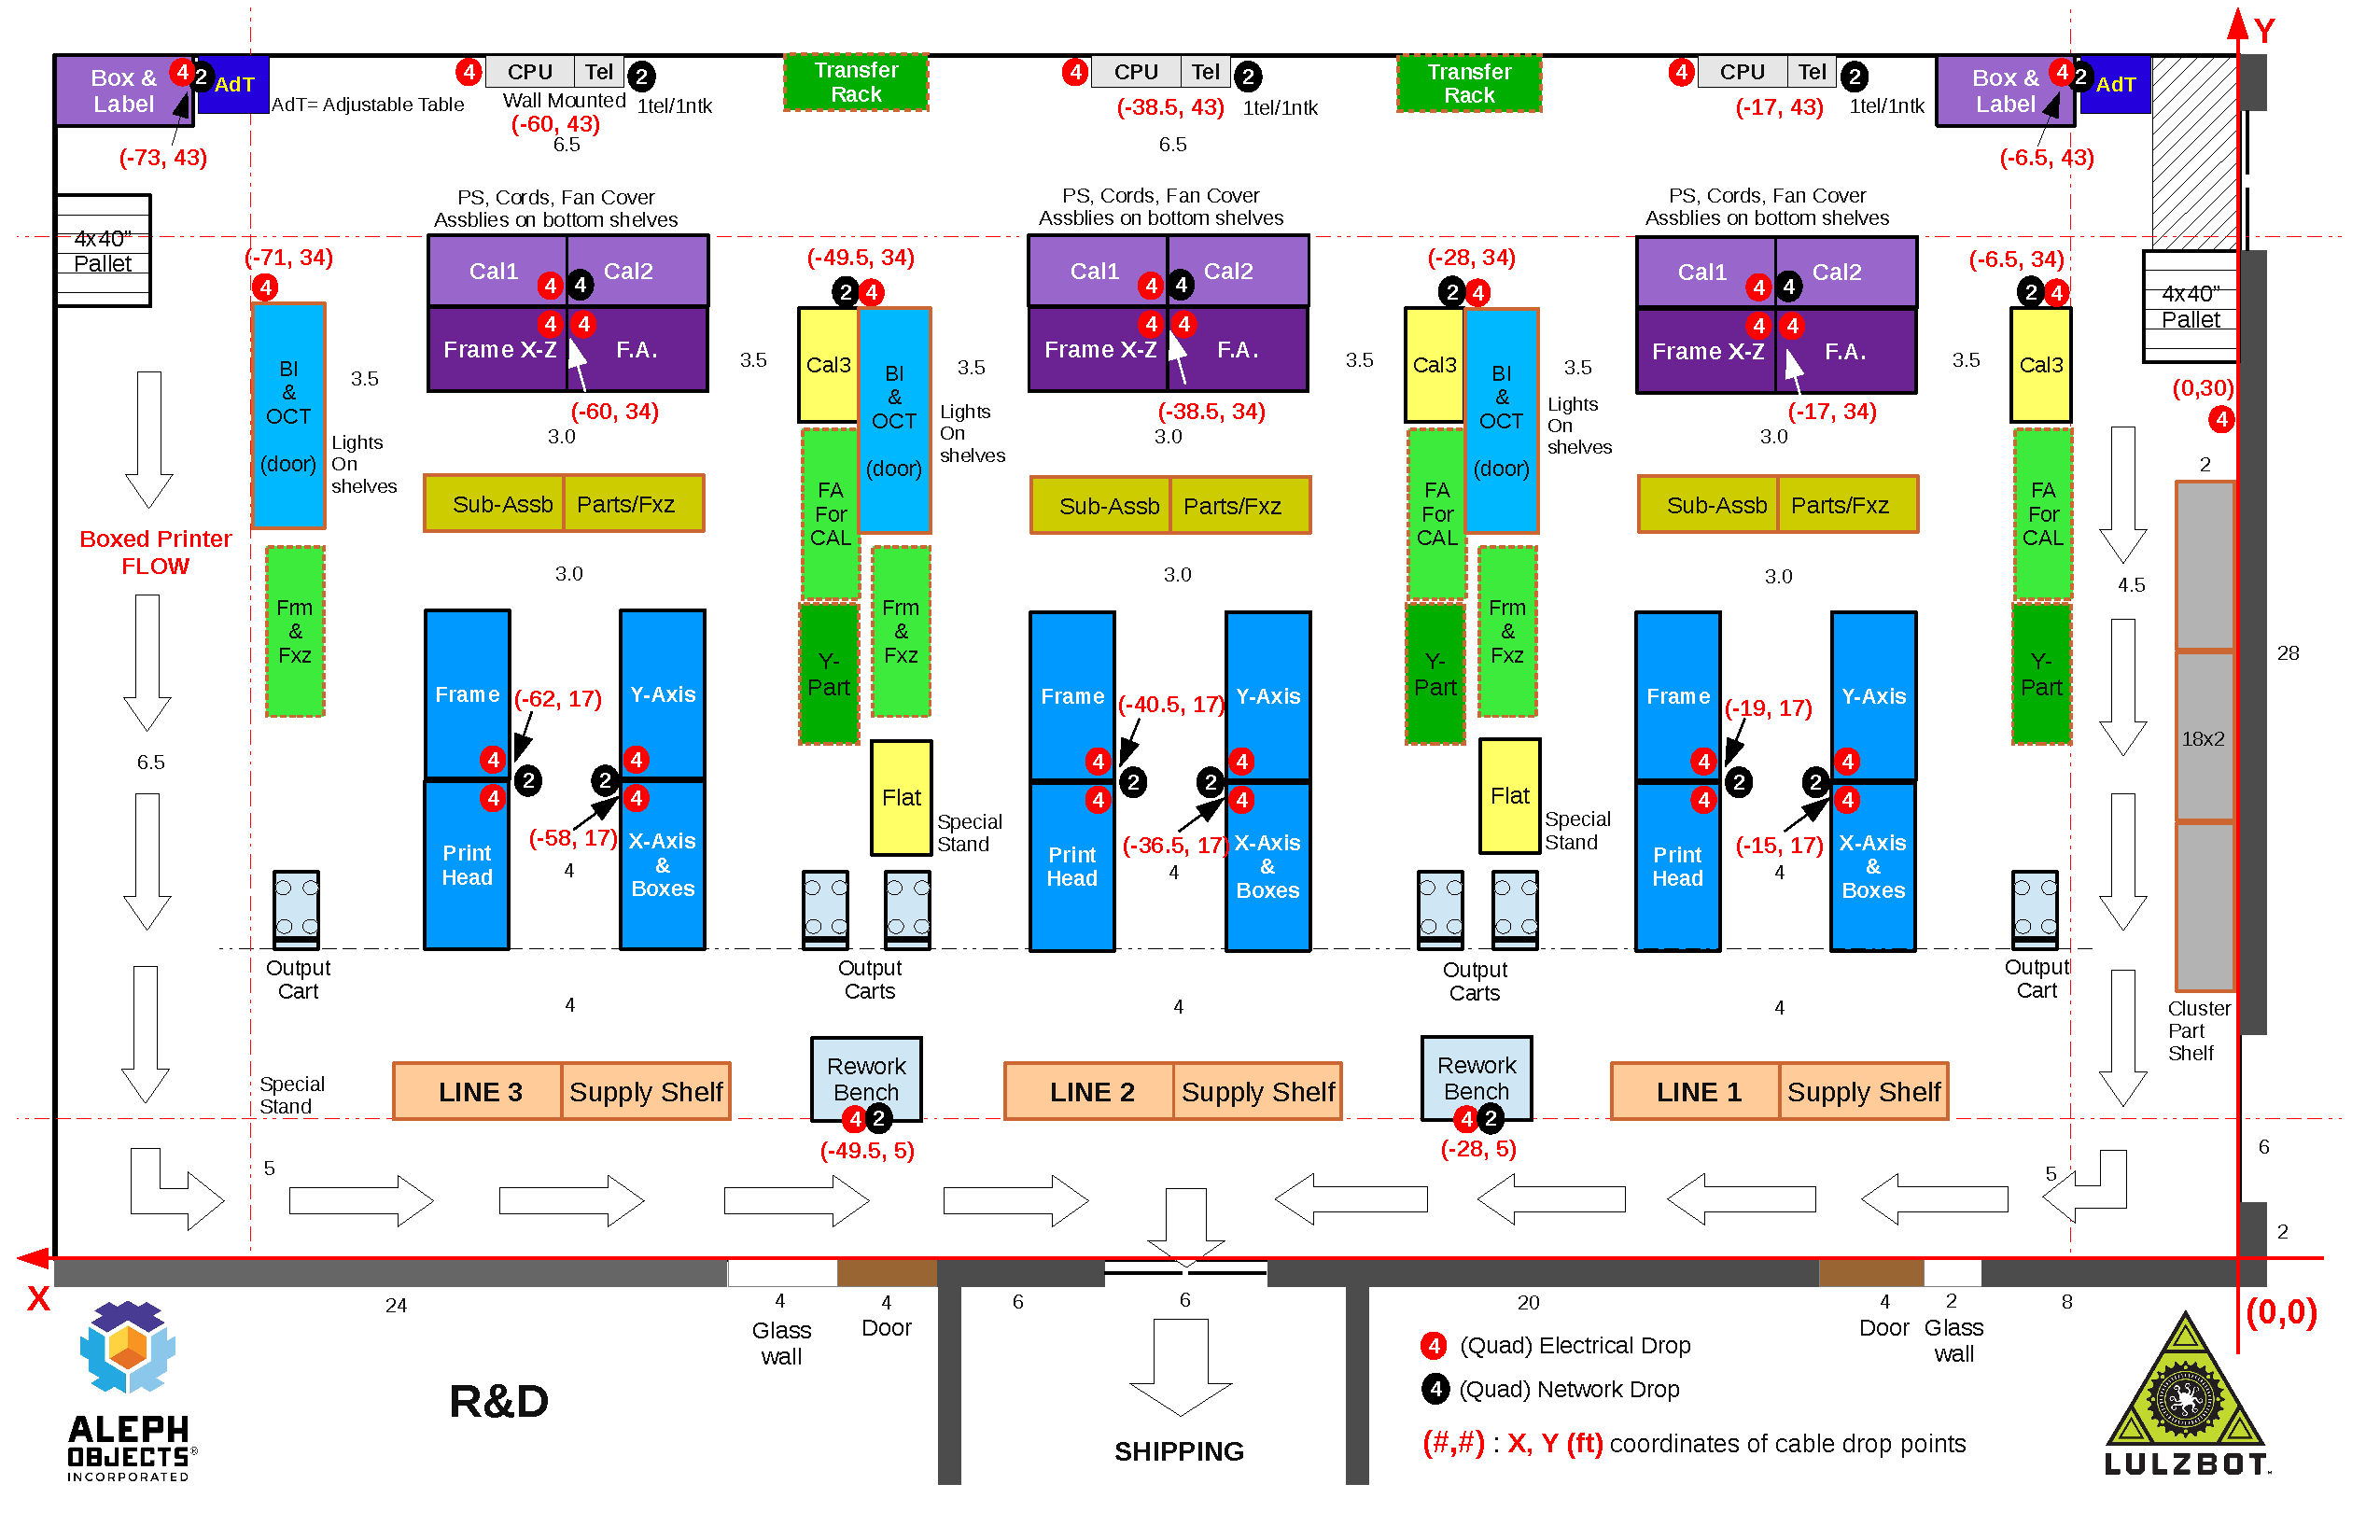
\includegraphics[keepaspectratio=true,angle=0,height=0.95\textheight,width=0.95\textwidth]{linelayout.pdf}
\end{center}
\caption{Main Line Layout}
 \label{fig:ao_linelayout}
\end{sidewaysfigure}


\section{Quality Control}
Link to docs here...

\section{Packaging}
Continually improve packaging. Lessen cost, very expensive at present.
Send to FedEx for testing.

\section{Lean}
Get rid of everything unused.
